\begin{figure}[h!]
\centering
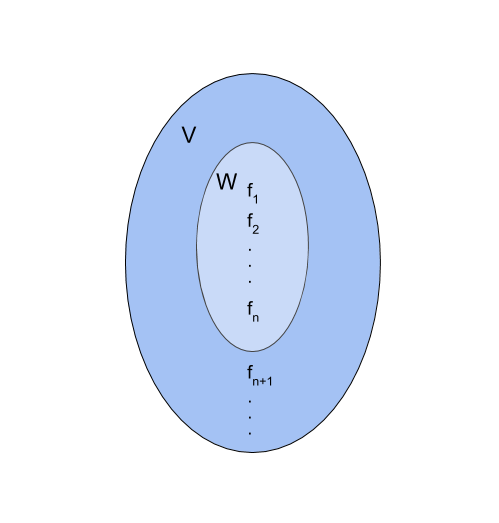
\includegraphics[scale=0.4]{solutions/3/6/3/fig/vector_space.png}
\caption{Vector space of all function $V$ and it's $n$-dimensional subspace $W$}
\label{eq:solutions/3/6/3/fig/1}
\end{figure}
%\pagebreak
\begin{figure}[h!]
\centering
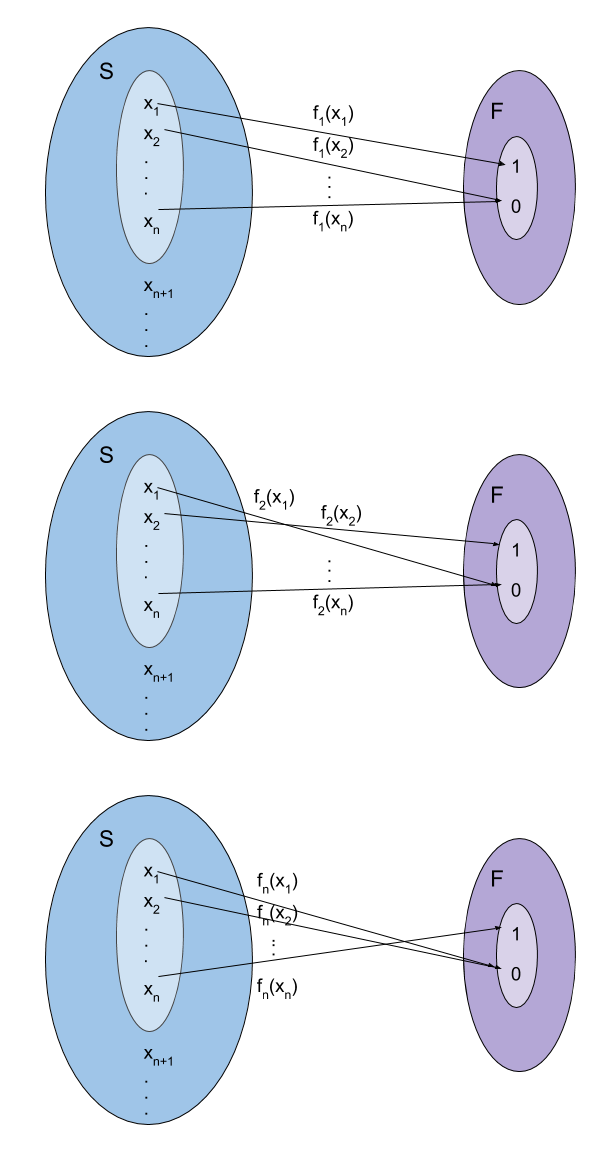
\includegraphics[width=\columnwidth]{solutions/3/6/3/fig/f.png}
\caption{Functions $f_1,f_2,\dots,f_n$ where $f:S \rightarrow F$ and $f_i(x_j) = \delta_{ij}$ for $i,j=1,\dots,n$}
\label{eq:solutions/3/6/3/fig/2}
\end{figure}

\begin{table}[h!]
\begin{center}
\begin{tabular}{|c|c|}
\hline
& \\
Given & $S$ is a set\\
& $F$ is a field\\
& $V(S,F)$ is a linear functional\\
& such that\\
& $W$ be $n$-dim subspace of $V(S,F)$.\\
& \\
& Also, \quad $\delta_{ij} = \begin{cases}1 \quad i=j\\ 0 \quad i \neq j \end{cases}$\\
& \\
\hline
& \\
To prove & $f_i(x_j) = \delta_{ij}$\\
& \\
& where $x_1, x_2, \dots, x_n \in S$\\
& and $f_1,f_2,\dots,f_n \in W$\\
& \\
\hline
& \\
Proof & Let $\phi_x : W \rightarrow F$\\
& \\
& Suppose $\phi_x(f) = 0 \enspace \forall x \in S \enspace \& \enspace f \in W$\\
& $\implies f(x) = 0$\\
& \\
& If $ \forall x, \enspace \phi_x(f) \neq 0 \enspace \text{for some } f \in W$\\
& If $n>0$ $\exists \in S$ such that\\
& $\phi_x(f) \neq 0$ for some $f \in W$\\
& $\implies f_1(x_1)\neq0$\\
& \\
& By scaling we can have\\
& $f_1(x_1) = 1$\\
& \\
& Hence $f_i(x_j) = \delta_{ij}$\\
& \\
\hline
\end{tabular}
\end{center}
\end{table}
{\em Example: }
\\
Consider points $\{x_1, x_2\} \in S$, let
\begin{align}
x_1&=1\\
x_2&=0
\end{align}
Also consider functions $\{f_1, f_2\} \in W$ where
\begin{align}
f_1(x) &= x\\
f_2(x) &= 1-x
\end{align}
Now, we have
\begin{align}
f_1(x_1) = f_1(1) = 1\\
f_1(x_2) = f_1(0) = 0
\end{align}
Also,
\begin{align}
f_2(x_1) = f_2(1) = 0\\
f_2(x_2) = f_2(0) = 1
\end{align}
Hence $f_i(x_j) = \delta_{ij}$.
\begin{figure}[h!]
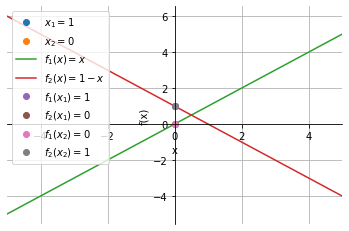
\includegraphics[width=\columnwidth]{solutions/3/6/3/fig/fig.png}
\caption{Functions $f_1,f_2$ and points $x_1,x_2$}
\label{eq:solutions/3/6/3/fig/3}
\end{figure}
